\documentclass{standalone}
\usepackage{tikz}
\usetikzlibrary{patterns, positioning}

\begin{document}
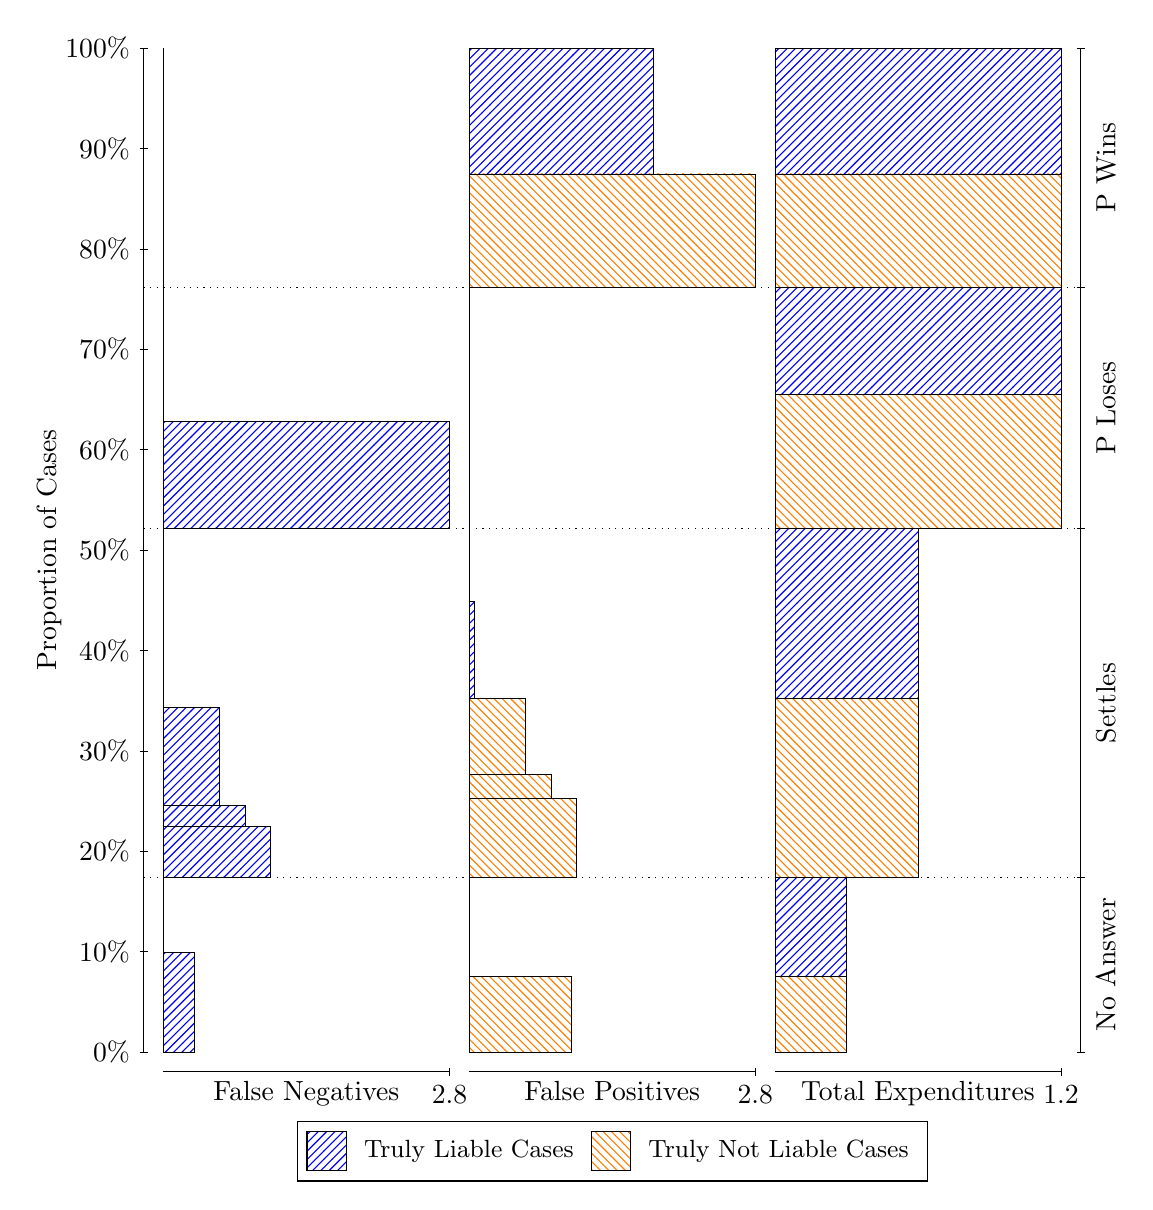
\begin{tikzpicture}
\draw[black, very thin] (1.5,1.75) -- (1.5,14.5);
\node[rotate=90, anchor=center] at (0.3, 8.125) {Proportion of Cases};
\draw[black, very thin] (1.45,1.75) -- (1.55,1.75);
\node[anchor=east] at (1.45, 1.75) {0\%};
\draw[black, very thin] (1.45,3.025) -- (1.55,3.025);
\node[anchor=east] at (1.45, 3.025) {10\%};
\draw[black, very thin] (1.45,4.3) -- (1.55,4.3);
\node[anchor=east] at (1.45, 4.3) {20\%};
\draw[black, very thin] (1.45,5.575) -- (1.55,5.575);
\node[anchor=east] at (1.45, 5.575) {30\%};
\draw[black, very thin] (1.45,6.85) -- (1.55,6.85);
\node[anchor=east] at (1.45, 6.85) {40\%};
\draw[black, very thin] (1.45,8.125) -- (1.55,8.125);
\node[anchor=east] at (1.45, 8.125) {50\%};
\draw[black, very thin] (1.45,9.4) -- (1.55,9.4);
\node[anchor=east] at (1.45, 9.4) {60\%};
\draw[black, very thin] (1.45,10.675) -- (1.55,10.675);
\node[anchor=east] at (1.45, 10.675) {70\%};
\draw[black, very thin] (1.45,11.95) -- (1.55,11.95);
\node[anchor=east] at (1.45, 11.95) {80\%};
\draw[black, very thin] (1.45,13.225) -- (1.55,13.225);
\node[anchor=east] at (1.45, 13.225) {90\%};
\draw[black, very thin] (1.45,14.5) -- (1.55,14.5);
\node[anchor=east] at (1.45, 14.5) {100\%};

\draw[black, very thin] (13.4,1.75) -- (13.4,14.5);
\draw[black, very thin] (13.35,1.75) -- (13.45,1.75);
\node[anchor=west] at (13.35, 1.75) {};
\draw[black, very thin] (13.35,3.9663) -- (13.45,3.9663);
\node[anchor=west] at (13.35, 3.9663) {};
\draw[black, very thin] (13.35,8.3969) -- (13.45,8.3969);
\node[anchor=west] at (13.35, 8.3969) {};
\draw[black, very thin] (13.35,11.463) -- (13.45,11.463);
\node[anchor=west] at (13.35, 11.463) {};
\draw[black, very thin] (13.35,14.5) -- (13.45,14.5);
\node[anchor=west] at (13.35, 14.5) {};

\draw[black, very thin, pattern color=blue, pattern=north east lines] (1.75,1.75) rectangle (2.1393,3.011);
\draw[black, very thin, pattern color=orange, pattern=north west lines] (1.75,3.011) rectangle (1.75,3.9663);
\draw[black, very thin, pattern color=blue, pattern=north east lines] (1.75,3.9663) rectangle (3.1125,4.6162);
\draw[black, very thin, pattern color=blue, pattern=north east lines] (1.75,4.6162) rectangle (2.7881,4.8838);
\draw[black, very thin, pattern color=blue, pattern=north east lines] (1.75,4.8838) rectangle (2.4637,6.1255);
\draw[black, very thin, pattern color=orange, pattern=north west lines] (1.75,6.1255) rectangle (1.75,8.3969);
\draw[black, very thin, pattern color=blue, pattern=north east lines] (1.75,8.3969) rectangle (5.3833,9.7548);
\draw[black, very thin, pattern color=orange, pattern=north west lines] (1.75,9.7548) rectangle (1.75,11.463);
\draw[black, very thin, pattern color=orange, pattern=north west lines] (1.75,11.463) rectangle (1.75,12.903);
\draw[black, very thin, pattern color=blue, pattern=north east lines] (1.75,12.903) rectangle (1.75,14.5);
\draw[black, very thin, pattern color=orange, pattern=north west lines] (5.6333,1.75) rectangle (6.931,2.7052);
\draw[black, very thin, pattern color=blue, pattern=north east lines] (5.6333,2.7052) rectangle (5.6333,3.9663);
\draw[black, very thin, pattern color=orange, pattern=north west lines] (5.6333,3.9663) rectangle (6.9958,4.9699);
\draw[black, very thin, pattern color=orange, pattern=north west lines] (5.6333,4.9699) rectangle (6.6714,5.272);
\draw[black, very thin, pattern color=orange, pattern=north west lines] (5.6333,5.272) rectangle (6.347,6.2377);
\draw[black, very thin, pattern color=blue, pattern=north east lines] (5.6333,6.2377) rectangle (5.6982,7.4794);
\draw[black, very thin, pattern color=blue, pattern=north east lines] (5.6333,7.4794) rectangle (5.6333,8.3969);
\draw[black, very thin, pattern color=orange, pattern=north west lines] (5.6333,8.3969) rectangle (5.6333,10.105);
\draw[black, very thin, pattern color=blue, pattern=north east lines] (5.6333,10.105) rectangle (5.6333,11.463);
\draw[black, very thin, pattern color=orange, pattern=north west lines] (5.6333,11.463) rectangle (9.2667,12.903);
\draw[black, very thin, pattern color=blue, pattern=north east lines] (5.6333,12.903) rectangle (7.969,14.5);
\draw[black, very thin, pattern color=orange, pattern=north west lines] (9.5167,1.75) rectangle (10.425,2.7052);
\draw[black, very thin, pattern color=blue, pattern=north east lines] (9.5167,2.7052) rectangle (10.425,3.9663);
\draw[black, very thin, pattern color=orange, pattern=north west lines] (9.5167,3.9663) rectangle (11.333,6.2377);
\draw[black, very thin, pattern color=blue, pattern=north east lines] (9.5167,6.2377) rectangle (11.333,8.3969);
\draw[black, very thin, pattern color=orange, pattern=north west lines] (9.5167,8.3969) rectangle (13.15,10.105);
\draw[black, very thin, pattern color=blue, pattern=north east lines] (9.5167,10.105) rectangle (13.15,11.463);
\draw[black, very thin, pattern color=orange, pattern=north west lines] (9.5167,11.463) rectangle (13.15,12.903);
\draw[black, very thin, pattern color=blue, pattern=north east lines] (9.5167,12.903) rectangle (13.15,14.5);
\draw[black, dotted] (1.5,3.9663) -- (13.4,3.9663);
\draw[black, dotted] (1.5,8.3969) -- (13.4,8.3969);
\draw[black, dotted] (1.5,11.463) -- (13.4,11.463);
\draw[black, very thin] (1.75,1.5) -- (5.3833,1.5);
\node[anchor=north] at (3.5667, 1.5) {False Negatives};
\draw[black, very thin] (5.3833,1.45) -- (5.3833,1.55);
\node[anchor=north] at (5.3833, 1.45) {2.8};

\draw[black, very thin] (5.6333,1.5) -- (9.2667,1.5);
\node[anchor=north] at (7.45, 1.5) {False Positives};
\draw[black, very thin] (9.2667,1.45) -- (9.2667,1.55);
\node[anchor=north] at (9.2667, 1.45) {2.8};

\draw[black, very thin] (9.5167,1.5) -- (13.15,1.5);
\node[anchor=north] at (11.333, 1.5) {Total Expenditures};
\draw[black, very thin] (13.15,1.45) -- (13.15,1.55);
\node[anchor=north] at (13.15, 1.45) {1.2};

\node[black, centered, rotate=90] at (13.72, 2.8581) {No Answer};
\node[black, centered, rotate=90] at (13.72, 6.1816) {Settles};
\node[black, centered, rotate=90] at (13.72, 9.9301) {P Loses};
\node[black, centered, rotate=90] at (13.72, 12.982) {P Wins};

\draw (7.449999999999999,1.5) node[draw=none] (baseCoordinate) {};
\begin{scope}[align=center]
        \matrix[scale=0.5, draw=black, below=0.5cm of baseCoordinate, nodes={draw}, column sep=0.1cm]{
            \node[rectangle, draw, minimum width=0.5cm, minimum height=0.5cm, pattern=north east lines, pattern color=blue] {}; &
            \node[draw=none, font=\small] (B) {Truly Liable Cases}; &
            \node[rectangle, draw, minimum width=0.5cm, minimum height=0.5cm, pattern=north west lines, pattern color=orange] {}; &
            \node[draw=none, font=\small] (B) {Truly Not Liable Cases}; \\
            };
\end{scope}

\end{tikzpicture}
\end{document}